\section{RC Circuits}

\begin{frame}{RC Circuits}
    The capacitor and resistor in a NOT circuit form the most basic RC circuit:
    
    Write down a differential equation describing the circuit below:
	\begin{center}
	    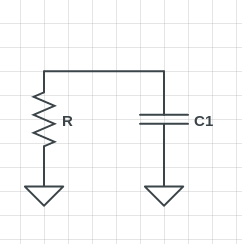
\includegraphics[width=0.5\textwidth]{./images/rc-circuits-1.png}
	\end{center}
\end{frame}

\begin{frame}{RC Circuits}
    The capacitor and resistor in a NOT circuit form the most basic RC circuit:
    
    Write down a differential equation describing the circuit below:
	\begin{center}
	    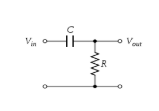
\includegraphics[width=0.5\textwidth]{./images/rc-circuits-2.png}
	\end{center}
\end{frame}

\begin{frame}{Solving the RC differential Equation}
    We have a differential equation describing $V_{out}$ in terms of \(V_c\).

    \[
        \frac{dV_c}{dt} = -\frac{1}{RC} V_c
    \]
    How do we actually solve it?

    \pause
    
    Think of the differential operation as a linear operator that scales $V_c$, since $V_c$ is one of its eigenfunctions:
	\[[\frac{d}{dt}]V_c = \lambda{V_c}\]
\end{frame}

\begin{frame}{Solving the RC differential Equation}
    Which are the eigenfunctions of differentiation?
    \pause
    
    \[Ae^{\lambda{t}}\]

    \pause
    
    \[\frac{dV_c}{dt} = -\frac{1}{RC}V_c\]
    
    The solution to our first order differential equations is therefore:

    \[V_c(t) = V_c(0)e^{\frac{-1}{RC}t} \]
\end{frame}

\begin{frame}{RC Differential Equation: Non-homogenous case}
	How do you solve a RC circuit with a voltage source?
    
    \begin{center}
    	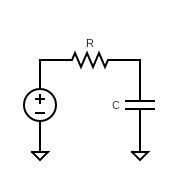
\includegraphics[width=0.2\textwidth]{./images/rc-circuits-3.png}
    \end{center}
    
    Applying KCL at the top right node, along with Ohm’s law and the capacitor relationship, we get:
    \[\frac{dV_c}{dt} = \frac{1}{VC}(V_s - V_c)\]
    
    We can't easily solve this equation, so we change variables to
    
    \[x = V_c - V_s\]
\end{frame}

\begin{frame}{RC Differential Equation: Non-homogenous case}
	Now, we have $\frac{dx}{dt} = -\frac{x}{RC}$
    
    We already know how to solve this differential equation, and we get                              
    \[
        x(t) = x_0e^{-\frac{t}{RC}}
    \]
    
    Finally, change back to the original variables by substituting $V_c$ - $V_s$ for $x$
    
    \[V_c(t) = V_c(0)e^{-\frac{t}{RC}} + V_s(1 - e^{-\frac{t}{RC}})\]
\end{frame}
